\chapter{Introduction}
This experiment aims to determine the lifetime of muons. Muons are produced by cosmic ray showers 
in the higher atmosphere. Incoming Protons react with the hadrons of the atmosphere and produce 
pions, which can decay into muons. Due to the high, relativistic velocities of the muons, they can 
reach the surface of the earth. \\
In this experimental setup the incoming muons are slowed down and stopped
by layers of iron and then detected with a plastic scintillator. A trigger logic is used to determine 
the lifetime of the various incoming muons.\\
This report is structured as follows: in this chapter an introduction into the physical aspects of muons is given.
\autoref{sec:setup} describes the used components and the experimental setup. In \autoref{sec:prem}
the preliminary measurements for the calibration of the setup are described and their results are discussed. \autoref{sec:trigger} discusses
the composition of the experiment and the process of data taking, while \autoref{sec:data_analysis} 
presents the the data analysis. \autoref{sec:results} concludes this report.

MAYBE MORE TEXT

\newpage
\section{General introduction to muons}
The standard model of elementary particles differentiates between quarks, leptons and bosons.
Quarks as well as leptons can be divides into three generations. The muons and the antimuon respectively 
are the second generation of leptons together with their each associated neutrinos. Like the electron,
muons have a spin $1/2$ and a negative elementary charge (a positive elementary charge for the antimuon).
Although the similarities, both leptons differ in regard to their masses and their lifetimes.\\
While the electron is a stable particle, the muon has a finite lifetime, whichs this experiment is supposed 
to detect. The lifetime, given as an average result of past measurements, is $\tau = \SI{2.1969811 \pm 0.0000022}{\micro\second}$.
Their mass is given as $m_{\mu} = \SI{105.6583745 \pm 0.0000024}{\mega\eV}$, which 
is 206 times the mass of the electron \cite{pdg}.
\section{Muons from cosmic ray showers} 
Muons are naturally produced in cosmic ray showers. When a particle strikes the 
hadrons in the upper atmosphere, they interact and produce a hadronic shower. These particles originate 
in various galactic and intergalactic sources like the sun, the Milky Way and other galaxies. The cosmic 
ray are mostly protons, but also electrons and atomic nuclei. The protons 
hadronize mostly into $\pi$ mesons, because they are the lightest mesons, but also into $K$ mesons 
and other hadrons.
The primary cosmic rays are completely hadronized at altitudes of $\SI{20}{km}$. Because $\pi$ mesons and $K$ mesons are not stable with lifetimes in the order of 
magnitude of $\SI{e8}{\second}$ they decay very fast. For the decay into muons, the $\pi$ mesons have a branching ratio
of $\Gamma = (99.98770\pm{0.00004})\%$, while the $K$ mesons have a branching ratio of $\Gamma = (63.56\pm{0.11})\%$ \cite{pdg}. 
It should be noted that these decays into muons only occure with charged $\pi$ and $K$ mesons. Neutral 
Mesons are also produced in these showers, but they do not decay into charged muons. The decay of the $\pi$ mesons 
takes place via the weak interaction 
\begin{align*}
    \pi^{+} &\to \mu^{+} + \nu_{\mu} \\
    \pi^{-} &\to \mu^{-} + \bar{\nu}_{\mu}.
\end{align*}
This process is analogous for $K$ mesons. The muons also only decay via the weak interaction as follows 
\begin{align*}
    \mu^{-} &\to e^{-} + \bar{\nu}_{e} \\
    \mu^{+} &\to e^{+} + \nu_{e}.
\end{align*}
Because the muons have a longer lifetime, they can reach the surface of the earth and can be detected through their decay. 
A scematic with typical processes, which lead among other things to the production of muon, can be seen in \autoref{fig:cosmic_ray_showers}.
\begin{figure}
    \centering
    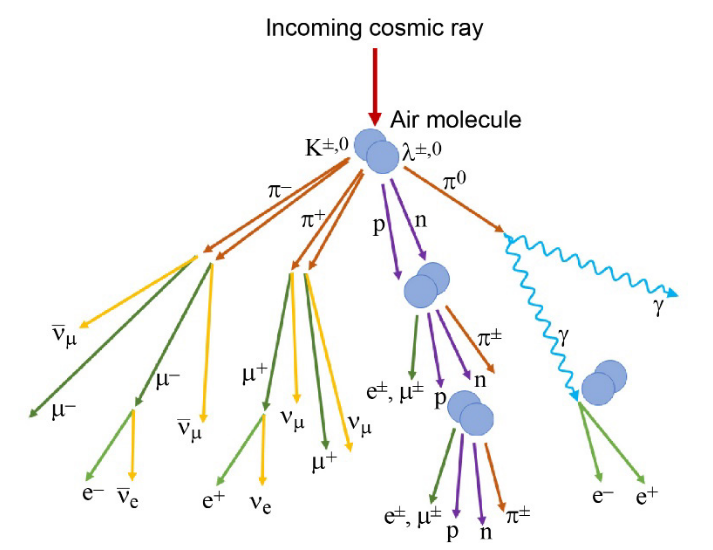
\includegraphics[width=0.67\textwidth]{figures/cascade.png}
    \caption{Typical shower processes after an incoming cosmic ray. The primary rays induce secondary particles by scatering with the 
    molecules of the atmosphere. These secondary can decay or scatter again with the atmosphere and producing more particles in the process. 
    This is called a decay chain or a cosmic ray shower\cite{nasa}.}
    \label{fig:cosmic_ray_showers}
\end{figure}